\chapter{Cinématique du point matériel}
\label{chap:cinematiquedupoint}
\minitoc
\minilof
\minilot

\section{Espace physique et temps d'un observateur}
\label{chap1-sec:espacephysique}

\subsection{Notion de solide}
\label{chap1-subsec:notion de solide}

En mécanique, certains corps physiques ont une forme indépendante des actions mécaniques qu'ils subissent. Ces corps sot appelés \emph{solides indéformables}. Les propriétés géométriques de l'ensemble des points d'un solide, tels que des distances ou des angles, sont invariants.

\subsection{Espace physique}
\label{chap1-subsec:espacephysique}

Jusqu'en 1960, le mètre était défini par une distance entre deux traits sur une barre de platine iridiée, qui s'appelle le \emph{mètre étalon}. On avait aussi définit le mètre comme un multiple de la longueur d'onde d'une certaine radiation de krypton.

Aujourd'hui ces définitions sont abandonnées et le mètre est défini tel que~:
\begin{defdef}
  Le mètre est la longueur du trajet que la lumière parcoure en une durée de $1/\numprint{299792458}$ secondes.
\end{defdef}

La mécanique classique et la relativité restreinte postulent que l'espace physique est un espace euclidien à trois dimensions. La relativité générale remet en cause cette hypothèse et postule plutôt que l'espace physique est un espace de Minkowski à quatre dimensions.

\subsection{Chronologie et définition de la seconde}
\label{chap1-subsec:chronologie}

La notion d'écoulement du temps est d'abord intuitive. Un observateur est tout à fait capable d'établir une chronologie. C'est-à-dire de déterminer si un événement à eu lieu avant ou après tel autre.

Le temps est un paramètre réel servant à dater les événements. N'importe quel instrument pouvant dater les événements constitue un chronomètre ou une horloge. Une personne qui énonce une suite de nombres ou un sablier sont des horloges.

Pour choisir parmi les différentes horloges, on impose une exigence supplémentaire~: l'uniformité du temps, ou, ce qui revient au même, nous postulons que \emph{les lois physiques sont invariantes par translation dans le temps}. Par exemple, si un pendule oscille en repassant toujours par les mêmes positions dans des conditions extérieures constantes, les lois physiques étant inchangées d'une oscillation à l'autre, la durée doit être la même pour chaque oscillation. On voit ainsi l'importance des phénomènes cycliques pour définir une chronologie.

Le problème crucial, dans l'exemple précédent comme pour toute horloge basée sur un phénomène cyclique, est celui des conditions extérieures qui doivent être constantes. Le choix d'une chronologie privilégiée permettant d'appliquer les lois de la mécanique s'est fait par des approximations successives. Les scientifiques ont longtemps utilisé l'astronomie pour définir l'unité de temps. 

Jusqu'en 1960, les scientifiques utilisaient le \emph{temps sidéral}. La seconde était définie comme la fraction $1/\numprint{86400}$ du jour sidéral (le jour sidéral est la durée que met une planète pour faire un tour sur elle-même par rapport aux étoiles, indépendamment de sa révolution autour du Soleil). L'inconvénient de cette définition est le suivant~: Le mouvement des astres s'accélérait sans qu'aucune explication plausible ne puisse être donnée. Alors qu'en réalité c'est le contraire~: la Terre ralentit à cause des frottements de l'eau des océans. C'était alors l'horloge qui retardait. Ensuite, les scientifiques ont utilisé le \emph{temps des éphémérides}, la révolution de la Terre autour du Soleil, pour définir la seconde. Aujourd'hui, on utilise plutôt des mesures de fréquence, qui sont très précises, pour définir la seconde. C'est le \emph{temps atomique}.
\begin{defdef}
  La seconde est la durée de $\numprint{9192631770}$ périodes de la radiation correspondant entre deux niveaux hyperfins de l'état fondamental de l'atome de césium 133.
\end{defdef}

\section{Mouvement et référentiel, temps absolu}
\label{chap1-sec:mvtetref}
\emph{Un référentiel d'espace-temps est un système d'axes de coordonnées attaché à un solide et muni d'une chronologie}. Du point de vue spatial, un référentiel est donc par définition indéformable, car les distances et les angles d'un ensemble de points du référentiel sont constants. Chaque référentiel d'espace-temps est muni d'une chronologie. On le muni d'une horloge atomique fixe dans le référentiel.

En mécanique classique, on considère que le temps est une notion indépendante du référentiel considéré. On parle dans ce cas de temps absolu, c'est-à-dire que des observateurs liés à des référentiels différents peuvent attribuer les mêmes dates aux mêmes événements.

La relativité restreinte remet en cause ce postulat. Le temps écoulé entre deux événements n'est pas le même dans deux référentiels d'espace-temps, munis d'horloges identiques, si le mouvement de l'un n'est pas une translation rectiligne uniforme par rapport à l'autre.

\section{Notion de point matériel}
\label{chap1-sec:notiondepointmateriel}

Un point matériel est un objet dont la position dans un référentiel donné est entièrement définie par ses trois coordonnées. Il ne suffit pas qu'un solide soit petit pour l'assimiler à un point matériel. Une molécule possédant un moment dipolaire possède une symétrie de révolution autour de son vecteur moment dipolaire mais pas la symétrie sphérique nécessaire. Il faudrait donc que l'objet que l'on assimile à un point matériel possède la symétrie sphérique du point géométrique et soit ainsi homogène et isotrope. Mais ceci ne suffit pas encore pour l'assimiler à un point matériel, le centre d'inertie d'une sphère homogène sur un plan incliné n'a pas le même mouvement selon qu'elle roule ou qu'elle glisse. Il faut donc de plus exclure pour un point matériel la possibilité de tourner.

Enfin, la condition de petitesse n'est même pas nécessaire. En effet, la Terre, dans l'étude du mouvement d'un satellite, peut être valablement être assimilée à un point matériel coïncident avec son centre d'inertie.

On appellera point matériel un corps, ou un point géométrique associé à un système de corps, dont la position géométrique est totalement déterminée par trois coordonnées. Le type même du point matériel est, comme on le verra, le point matériel fictif coïncidant avec le centre d'inertie d'un système, et où serait concentrée toute la masse du système.

\section{Complément de géométrie}
\label{chap1-sec:complementdegeometrie}

\subsection{Repère, coordonnées cartésiennes}
\label{chap1-subsec:reperecoord}

Un repère d'espace est constitué par un point et trois axes de coordonnées cartésiennes, qu'il soient ou non liés au référentiel auquel on rapporte le mouvement étudié.

En coordonnées cartésiennes, la position d'un point matériel est définie par son \emph{vecteur position} décomposable suivant la direction de ces trois axes~:
\begin{equation}
  \vv{OM}=x\vi+y\vj+z\vk=x\ux+y\uy+z\uz.
\end{equation}
Si le repère est lié au référentiel dans lequel on travail, ses axes sont considérés comme fixe. Les vecteurs unitaires de la base correspondante sont alors constants. Le déplacement élémentaire du point matériel est alors~:
\begin{equation}
  \D\vv{OM}=\D x\ux+\D y\uy+\D z\uz.
\end{equation}
La longueur de ce déplacement est donc~:
\begin{equation}
  \D s = ||\D\vv{OM}||,
\end{equation}
tel que
\begin{equation}
  (\D s)^2=(\D x)^2+(\D y)^2+(\D z)^2.
\end{equation}

\subsection{Coordonnées cylindriques, ou cylindro-polaires}
\label{chap1-subsec:coordcylindriques}

Un repère cartésien, que l'on supposera ici lié au référentiel dans lequel on étudie le mouvement, étant défini, les coordonnées cylindro-polaires sont les coordonnées polaires de la projection $H$ de $M$ dans le plan $(xOy)$~: la coordonnées radiale $\rho=r=\sqrt{x^2+y^2}$, l'angle polaire $\theta=(\vv{Ox}, \vv{OH})$ et la côte $z$.

Les vecteurs unitaires $\ur$, $\utheta$ et $\uz$ forment une base mobile utilisée pour décomposer les vecteurs. Par exemple
\begin{equation}
  \vv{OM}=r \ur + z\uz.
\end{equation}

On remarque que $\ur = \cos \theta \ux + \sin \theta \uy$ et $\utheta = -\sin \theta \ux + \cos \theta \uy$. D'autre part, $(Oxyz)$ étant un référentiel, les vecteurs $\ux$ et $\uy$ sont constants alors
\begin{equation}
  \derived{\ur}{\theta} = \utheta \quad \derived{\utheta}{\theta} = -\ur.
\end{equation}

Plus généralement, la dérivée d'un vecteur unitaire $\vu$ tournant dans un plan par rapport à l'angle qui définit sa direction dans ce plan est le vecteur $\vvv$ unitaire par rotation de $\vu$ de $\frac{\pi}{2}$.

 \begin{figure}
   \centering
   \begin{tikzpicture} [math3d]
     \draw (0,0,0) node[left, below] {$O$};    
     \coordinate (O) at (0,0,0);
     \coordinate (H) at (3,3,0);
     \coordinate (M) at (3,3,2);
     \draw [->] (O) -- ++(3,0,0) node[below] {$x$};
     \draw [->] (O) -- ++(0,3,0) node[right] {$y$};
     \draw [->] (O) -- ++(0,0,3) node[left] {$z$};
     \draw (O) -- (H) node[right] {$H$};
     \draw [->] (1.3,0,0) arc (0:55:1) node[right, above] {$\theta$};
     \draw (3,2,0) node[above] {$\rho$};
     \draw [dotted] (H) -- (M) node[left] {$M$};
     \draw [->] (M) -- ++(1,1,0) node[below] {$\ur$};
     \draw [->] (M) -- ++(-1,1,0) node[above] {$\utheta$};
     \draw [->] (M) -- ++(0,0,1) node[left] {$\uz$};
   \end{tikzpicture}
   \caption{Coordonnées cylindro-polaires}
   \label{fig:coordonnees}
 \end{figure}

\section{Trajectoire, abscisse curviligne et loi horaire}
\label{chap1-sec:trajectoireabcissecurv}

\emph{La trajectoire d'un point mobile dans un référentiel donné est l'ensemble des points de ce référentiel avec lesquels il coïncide successivement au cours du temps}. Il s'agit bien sûr d'une courbe continue. La trajectoire dépend du référentiel par rapport auquel on étudie le mouvement. Un sens positif noté par $\rightarrow s$ et une origine $A$ étant choisie arbitrairement sur la trajectoire, l'abscisse curviligne de $M$ est définie par $s=\overarc{AB}$. L'abscisse curviligne est une fonction du temps $t$ continue et dérivable. Cette fonction $f:t \rightarrow s=f(t)$ est appelée \emph{loi horaire du mouvement} ou équation horaire.

\section{Vitesse}
\label{chap1-sec:vitesse}

La vitesse d'un point matériel dans un référentiel où le point $O$ est fixe est
\begin{equation}
  v = \derived{\vv{OM}}{t}.
\end{equation}
Le point $O$ pouvant être remplacé par n'importe quel point lié au référentiel. On note encore la vitesse du point $M$ comme $\derived{\vv{M}}{t}$ ou $\dot{\vv{OM}}$ ou encore $\dot{\vv{M}}$. La vitesse est une fonction continue du temps. Si l'on utilise plusieurs référentiels, la vitesse de $M$ dans le référentiel $R$ est notée $\vec{v}_{M/R}$. Un déplacement élémentaire $\D \vv{M}$ du point $M$ est tangent à la trajectoire donc \emph{le vecteur vitesse est tangent à la trajectoire}.

Le vecteur $\ur$ étant tangent à la trajectoire et orienté dans le même sens que celle-ci, le déplacement élémentaire s'écrit $\D \vv{M}=\D s \vec{u}_T$ donc $\vv{v}=\dot{s} \vv{u}_T$, $\dot{s}$ est la \emph{vitesse algébrique} et \emph{la norme de la vitesse} est donc $v=|\dot{s}|$.

On appelle hodographe du mouvement la courbe décrite par l'extrémité du vecteur vitesse représenté avec une origine fixe.

En coordonnées cartésiennes,
\begin{equation}
  \vv{v} = \dot{x}\ux+\dot{y}\uy+\dot{z}\uz,
\end{equation}
et en coordonnées cylindriques $\dot{\ur}=\dot{\theta}\utheta$ et donc
\begin{equation}
  \vv{v}=\dot{r}\ur+r\dot{\theta}\utheta+\dot{z}\uz.
\end{equation}

\section{Accélération}
\label{chap1-sec:accélération}

L'accélération d'un point matériel dans un référetiel où le point $O$ est fixe est
\begin{equation}
  \vv{a}=\derived{\vv{v}}{t}=\deriveds{\vv{OM}}{t}.
\end{equation}
Elle peut présenter des discontinuités. Si l'on doit préciser le référentiel on note $\vv{a}_{M/R}$. Si la trajectoire n'est pas rectiligne, le vecteur unitaire tangentiel $\vec{u}_T$ varie donc sa dérivée par rapport au temps est normale à la trajectoire. Ainsi l'accélération a une composante tangentielle, $\ddot{s}$, et une composante normale à la trajectoire
\begin{equation}
  \vv{a}=\ddot{s}\vv{u}_T + \dot{s}\dot{\vv{u}_T}.
\end{equation}

En coordonnées cartésiennes,
\begin{equation}
  \vv{a} = \ddot{x}\ux+\ddot{y}\uy+\ddot{z}\uz,
\end{equation}
et en coordonnées cylindriques $\dot{\utheta}=-\dot{\theta}\ur$ et donc
\begin{equation}
  \vv{a}=(\ddot{r}-r\dot{\theta}^2)\ur+(2\dot{r}\dot{\theta}+r\ddot{\theta})\utheta+\ddot{z}\uz.
\end{equation}

Si $\vv{a}\cdot\vv{v}=\dot{s}\ddot{s}$ est positif, alors le mouvement est accéléré. Sinon alors le mouvement est ralenti.

\section{Mouvements particuliers}
\label{chap1-sec:mvtparticuliers}

\subsection{Lois horaires particulières}
\label{chap1-sec:loishorairespart}

Si $v=|\dot{s}|$ est constante on dit que le mouvement est uniforme et sa loi horaire est $s=\dot{s}t+s_0$.

Si $\ddot{s}$ est constant, le mouvement est dit uniformément varié. Alors la loi horaire s'écrit $s=\ddot{s} \frac{t^2}{2}+\dot{s}_0 +s_0$.

Un mouvement est sinusoïdal si $s=s_0+\alpha \cos(\omega t+\varphi)$. Le nombre $\alpha>0$ est l'amplitude du mouvement. Le nombre $\varphi$ est la phase à l'origine des dates. Le nombre $\omega>0$ est la pulsation ou fréquence angulaire du mouvement. Le mouvement est périodique de période $T=\frac{2\pi}{\omega}$ et de fréquence $f=\frac{1}{T}=\frac{\omega}{2\pi}$ (en Hertz). Un choix convenable de l'origine des dates et de l'origine des abscisses curvilignes permet de ramener cette loi horaire à la forme  $s = \alpha\cos(\omega t)$.

\subsection{Mouvements rectilignes}
\label{chap1-sec:mvtrect}

Pour un mouvement rectiligne, $\vv{u}_T$ est constant, l'accélération est tangentielle~: $\vv{a}=\ddot{s} \vv{u}_T$. On choisit l'axe $(Ox)$ suivant la trajectoire ($s$ est alors noté $x$ et l'origine des abscisses curvilignes est en $O$). La loi horaire est alors $f:t \rightarrow x=f(t)$.

Si le mouvement est rectiligne uniforme alors $\vv{v}$ est constant et l'accélération est nulle.

Si le mouvement est rectiligne uniformément varié alors $\vv{a}$ est constant. La réciproque est fausse.

Si le mouvement est rectiligne sinusoïdal, avec le choix de $O$ au milieu du segment parcouru, la loi horaire s'écrit $x=X\cos(\omega t+\varphi)$ ou $x=A\cos(\omega t) + B\sin(\omega t)$. L'accélération s'écrit $\vv{a}=-\omega^2X\cos(\omega t+\varphi)=-\omega^2 \vv{OM}$.

Si à $t=0$, on a
\begin{equation}
  x=x_0=X\cos(\varphi) \quad \dot{x}=\dot{x}_0=-\omega X\sin(\varphi),
\end{equation}
alors
\begin{equation}
  X=\sqrt{x_0^2+\frac{\dot{x}_0^2}{\omega^2}} \quad \tan(\varphi)=-\frac{\dot{x}_0}{\omega x_0}.
\end{equation}
Si $x_0>0$ alors $\varphi=-\arctan\left(\frac{\dot{x}_0}{\omega x_0}\right)$, sinon $\varphi=\pi-\arctan\left(\frac{\dot{x}_0}{\omega x_0}\right)$.

On obtient plus directement $A$ et $B$ avec $x_0=A$ et $\dot{x}_0=\omega B$.

\subsection{Mouvements à accélération constante}
\label{chap1-subsec:accelerationcst}

Si $\vv{a}$ est constant, alors $\vv{v}=\vv{v_0}+\vv{a}t$ et $\vv{OM}= \vv{OM}_0+ \vv{v_0} t + \vv{a}\frac{t^2}{2}$ .

On choisit les axes du repère avec $M_0=O$ comme origine, l'axe $Oz$ parallèle à l'accélération $\vv{a}$ et de sens contraire et le plan $(xOz)$ confondu avec le plan $(\vv{a},\vv{v_0})$.

On a donc, avec $\alpha=(\vv{Ox},\vv{v_0})$~:
\begin{align}
  \vv{a}&=\ddot{z} \uz=-a\uz \\
  \vv{v_0}&=\dot{x}\ux+\dot{z}\uz=v_0\cos\alpha\ux+v_0\sin\alpha\uz.
\end{align}
On en déduit
\begin{equation}
  \begin{cases}
    x&=v_0 t \cos\alpha\\
    y&=0\\
    z&=-\frac{a}{2}t^2+v_0 t \sin\alpha.
  \end{cases}
\end{equation}

En éliminant la date $t=\frac{x}{v_0\cos\alpha}$, on obtient l'équation de la trajectoire~:
\begin{equation}
  z = -\frac{a}{2v_0^2\cos^2\alpha}x^2+x\tan\alpha,
\end{equation}
c'est l'équation d'une parabole, représentée sur la figure \ref{fig:acceleration_constante}. La limite des points atteignables à accélération et vitesse initiale figées est la courbe d'équation $z_{max} = \frac{z_l}{2} - \frac{x^2}{2 z_l}$ avec $z_l = v_0^2/a$.

% TODO: \usepackage{graphicx} required
\begin{figure}
	\centering
	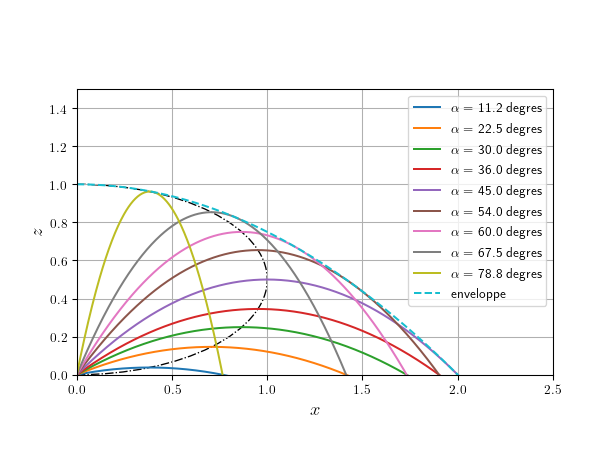
\includegraphics[width=0.8\linewidth]{acceleration_constante}
	\caption{Mouvement à accélération constante avec $a = g = \SI{9,81}{m/s^2}, v_0=\SI{20}{m/s}$}
	\label{fig:acceleration_constante}
\end{figure}

\emph{La trajectoire d'un point matériel dont l'accélération est constante est une parabole}. Le mouvement de la projection de $M$ sur $(Ox)$ est uniforme et celui de la projection de $M$ sur $Oz$ est uniformément varié. Si $\vv{v_0}$ et $\vv{a}$ sont parallèles alors le mouvement de $M$ est rectiligne uniformément varié sur l'axe $Oz$.

Avec les équations vectorielles on démontre facilement les propriétés suivantes~:
\begin{itemize}
\item la vitesse moyenne entre $t_1$ et $t_2$ est égale à la vitesse à $\frac{t_1+t_2}{2}$
  \begin{equation}
    \vv{v}_{1,2}=\vv{v}_{\left(\frac{t_1+t_2}{2}\right)}=\frac{\vv{v}_1+\vv{v}_2}{2};
  \end{equation}
\item la variation du carré de la vitesse est le double du produit scalaire de l'accélération par le vecteur déplacement
  \begin{equation}
v_2^2-v_1^2=2\vv{a}\cdot \vv{M_1M_2};
  \end{equation}
\item les vecteurs déplacements pendant des intervalles de temps successifs de même durée $\tau$ forment une suite arithmétique~:
  \begin{equation}
    \vv{M_nM_{n+1}}-\vv{M_{n-1}M_{n}}=\vv{a}\tau^2
  \end{equation}
\end{itemize}

\subsection{Mouvements circulaires}
\label{chap1-subsec:mvtcirc}

% \begin{figure}
%   \centering
%   \begin{tikzpicture}
%     \coordinate (O) at (0,0);
%     \coordinate (A) at (0,6);
%     \coordinate (B) at (6,0);
%     \coordinate (M) at (120:4);
%     \draw (0,0) node[below]{$\vv{\omega} \ Oz$};
%     \draw[>=latex] (0,0) circle(4);
%     \draw[->] (O) -- (B) node[below]{$x$};
%     \draw[->] (O) -- (A) node[left]{$y$};
%     \draw (O) -- (M) node[right]{$M$};

%     \draw[>=latex, ->] (M) -- ++(120:1) node[above]{$\urho$};
%     \draw[>=latex, ->] (M) -- ++(210:1) node[below]{$\utheta$};
    
%   \end{tikzpicture}
%   \caption{Mouvement circulaire}
%   \label{fig:mvt-circulaire}
% \end{figure}

Un point matériel mobile $M$ se meut circulairement s'il ce déplace sur un cercle. Dans ce cas, il est pratique d'utiliser les coordonnées polaires.

En notant $R$ le rayon du cercle parcouru par $M$ et $O$ son centre, si $s=0$ lorsque $\theta=0$ alors $s=R\theta$, $\dot{s}=R\dot{\theta}$ et $\ddot{s}=R\ddot{\theta}$.

Le vecteur \emph{vitesse angulaire} est $\vv{\omega}=\dot{\theta}\uz$. Sa norme vaut $\omega=\frac{v}{R}$ et elle s'exprime en $\si{rad\per s}$. 

Le vecteur vitesse est 
\begin{equation}
 \vv{v}=\dot{s}\utheta=R\dot{\theta} \utheta= \vv{\omega} \wedge \vv{OM}.
\end{equation}
C'est le moment en $M$ du vecteur vitesse angulaire représenté en $O$.

Le vecteur accélération est
\begin{equation}
\vv{a}=-R\dot{\theta}^2\ur +R\ddot{\theta}\utheta=-\frac{v^2}{R}\ur+\ddot{s}\utheta.  
\end{equation}
On constate que l'accélération normale est orientée vers le centre du cercle.

Si le mouvement est circulaire uniforme, alors l'accélération angulaire $\ddot{\theta}$ est nulle. Le vecteur vitesse angulaire $\vv{\omega}$ est constant, l'accélération est donc normale~:
\begin{equation}
  \vv{a}=-R\dot{\theta}^2\ur =-\omega^2\vv{OM}.
\end{equation}
Le mouvement est périodique de période $T=\frac{2\pi}{\omega}=\frac{2\pi R}{v}$ et de fréquence $f=\frac{1}{T}=\frac{\omega}{2\pi}=\frac{v}{2\pi R}$.

\section{Produit vectoriel}
\label{chap1-sec:produitvectoriel}

\subsection{Définition}
\label{chap1-subsec:defprodvec}

Soit la base $(\vu,\vvv,\vw)$ formant un trièdre direct. Soient deux vecteurs $\vU$ et $\vV$ de coordonnées respectives dans cette base $(U_1,U_2,U_3)$ et $(V_1,V_2,V_3)$. Le produit vectoriel est donné par
\begin{equation}
  \vU \wedge \vV = (U_2V_3-U_3V_2) \vu + (U_3V_1-U_1V_3) \vvv + (U_1V_2-U_2V_1) \vw
\end{equation}

\subsection{Propriétés du produit vectoriel}
\label{chap1-subsec:propprodvec}

Le produit vectoriel est une loi de composition interne dans $\R^3$. Il est anticommutatif $\vU\wedge\vV=-\vV\wedge\vU$. Il n'est pas associatif, ce qui peut être constaté avec la formule du double produit vectoriel
\begin{equation}
  \label{eq:doubleproduitvectoriel}
  (\vU\wedge\vV)\wedge\vW=(\vU\cdot\vW)\vV-(\vV\cdot\vW)\vU,
\end{equation}
et il est distributif à gauche et à droite par rapport à la somme
\begin{gather}
  \vU\wedge(\vV+\vW)= \vU\wedge\vV + \vU\wedge\vW;\\
  (\vU+\vV)\wedge\vW = \vU\wedge\vV + \vU\wedge\vW.
\end{gather}

\subsection{Norme, direction et sens du produit vectoriel, produit vectoriel nul}
\label{chap1-sec:normedirectionetsensproduitvectoriel}

En choisissant $(xOy)$ suivant le plan défini par les deux vecteurs avec $(O\vv{x})$ dans la direction et le sens de $\vU$, si $(\vU,\vV)=\alpha$, leurs coordonnées sont, dans la base $(\ex,\ey,\ez)$ formant un trièdre trirectangle de sens direct~: $(U,0,0)$ et $(V\cos\alpha,V\sin\alpha,0)$. On a alors $\vU\wedge\vV = UV\sin\alpha\ez$. Le trièdre $(\vU,\vV,\vU\wedge\vV)$ est de sens direct.

Le produit vectoriel est nul si et seulement si la famille $(\vU,\vV)$ est liée, c'est-à-dire si et seulement s'ils sont colinéaires ou l'un des deux est nul.

\subsection{Moment en un point d'un vecteur lié}
\label{chap1-sec:momentenunpointdunvecteurlié}

On appelle vecteur lié un vecteur représentant une caractéristique physique d'un point donné (vitesse, accélération, force subie, \ldots) et on le représente alors en ce point.

Le moment en $P$ du vecteur $\vU$ lié au point $M$ est par définition
\begin{equation}
  \Mom{P}{\vU}=\vv{PM}\wedge\vU.
\end{equation}

\section{Exercices}
\label{chap1-sec:exercices}
\begin{exercice}[Mouvements uniformément variés]
  Démontrer que dans un mouvement uniformément varié d'accélération tangentielle $\ddot{s}$,
  \begin{enumerate}
  \item les distances parcourues pendant des intervalles de temps successifs de même durée $\tau$ forment une suite arithmétique de raison $\ddot{s}\tau^2$;
  \item la variation du carré de la vitesse entre $t_1$ et $t_2$ s'exprime par
    \begin{equation}
      \dot{s}_2^2-\dot{s}_1^2 = 2 \ddot{s}(s_2-s_1),
    \end{equation}
  \item la vitesse algébrique moyenne entre $t_1$ et $t_2$ est égale à la vitesse algébrique en $\frac{t_1+t_2}{2}$ et à la moyenne des vitesses algébriques à $t_1$ et $t_2$.
  \end{enumerate}
\end{exercice}
%
\begin{exercice}[Exemple de mouvement circulaire]
  Un point $M$ se déplace sur un cercle de centre $O$ et de rayon $R=\SI{1}{m}$. Sa position est repérée par l'angle $\theta=(\vv{OM_0},\vv{OM})$ et la loi horaire de ce mouvement est $\theta=\pi\sin\left(\frac{2\pi t}{T}\right)$ avec une période de $T=\SI{1}{s}$.
  \begin{enumerate}
  \item À quelle date le mobile $M$ passe-t-il pour la première fois en $M_1$ d'angle polaire $\theta_1=\frac{\pi}{2}$ ?
  \item Calculez numériquement les coordonnées radiale et orthoradiale du vecteur vitesse à la date $t_1$ à laquelle $M$ est en $M_1$.
  \item Même question pour l'accélération.
  \item Pour quelles valeurs de $\theta$ la norme du vecteur accélération est-elle maximale ?
  \end{enumerate}
\end{exercice}
%
\begin{exercice}[Roulement sans glissement, cycloïde]
  Une roue de rayon $R$, de centre $C$, roule sans glisser sur l'axe $(Ox)$. Le mouvement de la roue est paramétrée par l'angle $\theta$ dont la roue à tourné depuis l'instant initial $t=0$ où l'abscisse de $C$ était nulle.
  \begin{enumerate}
  \item Quelles sont, en fonction de $R$ et de $\theta$, les coordonnées du point $M$ de la périphérie de la roue qui coïncidait avec le point $O$ à la date $t=0$ ?
  \item Calculez, en fonction de $R$ et de $\theta$ et des ses dérivées temporelles, les composantes de la vitesse et de l'accélération de $M$.
  \item Donnez les valeurs de la vitesse et de l'accélération de $M$ au moment où ce point touche l'axe $(Ox)$.
  \end{enumerate}
\end{exercice}
%
\begin{exercice}[Courbes de Lissajous]
  Les coordonnées cartésiennes d'un point sont données en fonction du temps par
  \begin{equation}
    \begin{cases}
      x(t) &= a\sin(\omega_1 t)\\
      y(t) &= b\sin(\omega_2 t)
    \end{cases}.
  \end{equation}
  \begin{enumerate}
  \item Quelle relation doit exister entre $\omega_1$ et $\omega_2$ pour que la trajectoire soit fermée ?
  \item Tracez cette trajectoire pour $\frac{\omega_2}{\omega_1}=\frac{3}{2}$.
  \end{enumerate}
\end{exercice}
%
\begin{exercice}[Spirale logarithmique]
  Trois chats se trouvent initialement aux sommets d'un triangle équilatérale. Le premier court après le second qui poursuit le troisième, lui-même courant après le premier. Ils courent à la même vitesse et celle-ci reste constante pendant toute la poursuite.
  \begin{enumerate}
  \item Déterminez la durée de la poursuite.
  \item Déduisez-en la distance parcourue par chacun des chats.
  \item Déterminez l'équation de la trajectoire de l'un des chats en coordonnées polaires.
  \end{enumerate}
\end{exercice}
%
\begin{exercice}[Mouvement uniforme sur une astroïde]
  Un homme partant du point $O$ à $t=0$ décrit l'axe $Oy$ avec une vitesse constante $W$. Son chien part du point $A$, d'abscisse $a$ sur l'axe $(Ox)$, se dirige constamment vers lui à la vitesse constante $2W$.
  \begin{enumerate}
  \item Quelle est la trajectoire $y=f(x)$ du chien ? Tracez l'allure de cette courbe.
  \item À quelle ordonnée le chien rejoint-il l'homme ? Quelle distance a-t-il parcourue ? À quelle date rejoint-il l'homme ?
  \item On note $H$ la position de l'homme et $Hx$ et $Hy$ les parallèles à $(Ox)$ et $Oy$ d'origine $H$. Établissez l'équation $r=g(\theta)$ de la trajectoire en coordonnées polaires dans le repère $Hx,Hy$. Tracez l'allure de cette trajectoire.
  \end{enumerate}
\end{exercice}